\chapter{Pendahuluan}

\section{Latar Belakang}
\label{sec:latarbelakang}

Transaksi pembayaran merupakan bagian penting dari aktivitas ekonomi, baik dalam lingkup individu maupun organisasi. Proses ini mencakup pengalihan dana antara pihak yang terlibat untuk memenuhi kewajiban finansial. Dalam perkembangannya, metode pembayaran telah bertransformasi dari yang awalnya menggunakan uang tunai dan cek menjadi transfer bank dan sistem yang lebih modern berbasis digital. Transformasi ini bertujuan untuk meningkatkan efisiensi, keamanan, dan kenyamanan dalam melakukan transaksi.

\qrisfull{} menjadi salah satu faktor pesatnya perkembangan teknologi pembayaran digital di Indonesia. \qris{} diluncurkan oleh Bank Indonesia pada tahun 2019 dan menjadi metode pembayaran yang populer dalam waktu kurang dari lima tahun karena kemudahan dan efisiensinya. Generasi Z dan millenial, sebagai pengguna utama metode pembayaran ini, merasakan kemudahan dalam melakukan pembayaran atau pengeluaran uang. Goodstats menunjukkan bahwa 38\% Gen Z menggunakan \qris{} dalam kehidupan sehari-hari, sementara di kalangan millenial angkanya mencapai 
25\%. 

Pada April 2024, Bank Indonesia melaporkan jumlah pengguna \qris{} mencapai angka 48,12 juta dan jumlah merchant yang menggunakan mencapai 31,61 juta. Total nilai transaksi dengan menggunakan metode pembayaran \qris{} telah mencapai Rp 31,65 triliun, yaitu meningkat sebesar 149,46\% secara tahunan 
pada bulan Februari 2024. Peningkatan ini mencerminkan adopsi yang signifikan di kalangan masyarakat, khususnya Gen Z dan millenial, yang cenderung memilih 
transaksi non-tunai. Survei dari Jawa Pos Radar Lawu mengungkapkan bahwa 57\% dari kedua generasi ini lebih memilih transaksi non-tunai, dengan \qris{} menjadi salah satu metode yang paling efektif. 

\newpage

Kemudahan ini mendorong peningkatan frekuensi transaksi digital di kalangan pengguna yang mengakibatkan kenaikan pada angka volume transaksi. Namun, seiring dengan meningkatnya volume transaksi, belum terdapat sistem dengan mekanisme pencatatan transaksi yang akurat dan cepat. Banyak pengguna masih harus melakukan pencatatan manual untuk memantau pengeluaran mereka yang rentan terhadap kesalahan dan memakan waktu. Salah satu solusi potensial untuk masalah ini adalah penerapan teknologi berbasis \cvfull{} dan \dl{} yang dapat melakukan pemindaian dan ekstraksi data dari dokumen gambar secara akurat, seperti \ocrfull, \cnnfull, \transformer, dan lainnya.

\layoutlm{} dan \bert{} merupakan model transformer yang menggabungkan informasi visual dan tekstual untuk memahami dokumen. Namun, kedua model ini masih bergantung pada \ocr. Ketergantungan ini membuat kedua model tersebut kurang efisien. Oleh karena itu, sistem yang dapat mengonversi dan mengekstrasi data dari bukti pembayaran berbasis kertas menjadi dokumen digital yang tidak bergantung pada OCR menjadi sistem yang diperlukan. 

\section{Rumusan Masalah}

Berdasarkan latar belakang dan masalah yang dihadapi oleh individu untuk melakukan pengelolaan bukti dan struk pembayaran, dapat dirumuskan masalah yang akan diselesaikan adalah sebagai berikut.

\begin{center}
	"Bagaimana cara mengonversi dan mengektraksi data dari bukti dan struk pembayaran yang berbasis kertas dan bervariasi menjadi dokumen digital?"
\end{center}

\section{Tujuan}

Penelitian ini bertujuan untuk mengembangkan sistem berbasis \emph{computer vision} dan \dl untuk memindai, mengonversi, dan mengekstrak data dari bukti pembayaran dengan format yang berbeda-beda secara akurat dan cepat untuk mendukung pencatatan dan pengelolaan transaksi keuangan secara digital

\section{Batasan Masalah}

Dalam pemenuhan solusi untuk menjawab masalah yang ada, terdapat berbagai jenis batasan yang perlu dipertimbangkan. Batasan-batasan tersebut ditentukan berdasarkan jangka waktu yang tersedia dan lingkup masalah yang akan diselesaikan. Berikut adalah batasan selama pengerjaan tugas akhir ini:
\begin{enumerate}
	\item Sistem hanya dapat memproses dokumen keuangan, seperti bukti pembayaran QRIS, transfer, dan struk yang dicetak dan tidak ditulis 
	\item Dokumen keuangan yang diterima hanya dalam format gambar digital dengan format JPG, JPEG, atau PNG dengan kualitas gambar yang jelas dan tidak blur. 
	\item  Pengembangan sistem dibatasi untuk memproses dokumen dari bank-bank digital ternama, yaitu SeaBank dan Neobank, bank-bank konvensional ternama, yaitu BCA dan BNI, aplikasi pembayaran digital populer, yaitu ShopeePay, OVO, dan Gopay.
	\item  Proses ekstraksi data dari struk pembayaran dibatasi pada informasi esensial transaksi yaitu:  
	\begin{itemize}
		\item Nominal pembayaran 
		\item ID transaksi 
		\item Aplikasi pembayaran 
		\item Penerima pembayaran
		\item Tanggal dan waktu transaksi 
	\end{itemize}
	\item Sistem dikembangkan untuk memproses satu dokumen bukti pembayaran dalam satu waktu.
	\item Pengujian sistem akan dilakukan dengan dataset minimal 100 sampel bukti pembayaran yang dikumpulkan dengan memperhatikan variasi sampel bukti pembayaran.
	\item Sistem dirancang untuk beroperasi dalam \emph{platform mobile} Android dan tidak mencakup pengembangan untuk \emph{platform desktop} atau iOS.
	\item Implementasi tidak mencakup integrasi dengan sistem akuntansi atau sistem pencatatan keuangan pihak ketiga.
	\item Pengembangan antarmuka pengguna dibatasi pada fitur-fitur dasar yang diperlukan untuk mengunggah gambar, memroses, dan menampilkan hasil ekstraksi data.
\end{enumerate}

\section{Metodologi}

Metodologi yang akan digunakan pada tugas akhir ini adalah \crispfull. Metodologi \crisp{} adalah kerangka kerja standar yang dirancang untuk memandu proses analisis data dan pengembangan solusi berbasis data secara sistematis (Saltz 2021). \crisp{} menjadi metodologi yang cocok untuk digunakan karena melibatkan proses pengolahan data yang sistematis dan iteratif, khususnya untuk mengembangkan solusi untuk menjawab rumusan masalah yang telah didefinisikan sebelumnya. Tahapan \crisp{} tergambar pada \autoref{fig:crisp-dm}.

\begin{figure}[htbp]
	\centering
	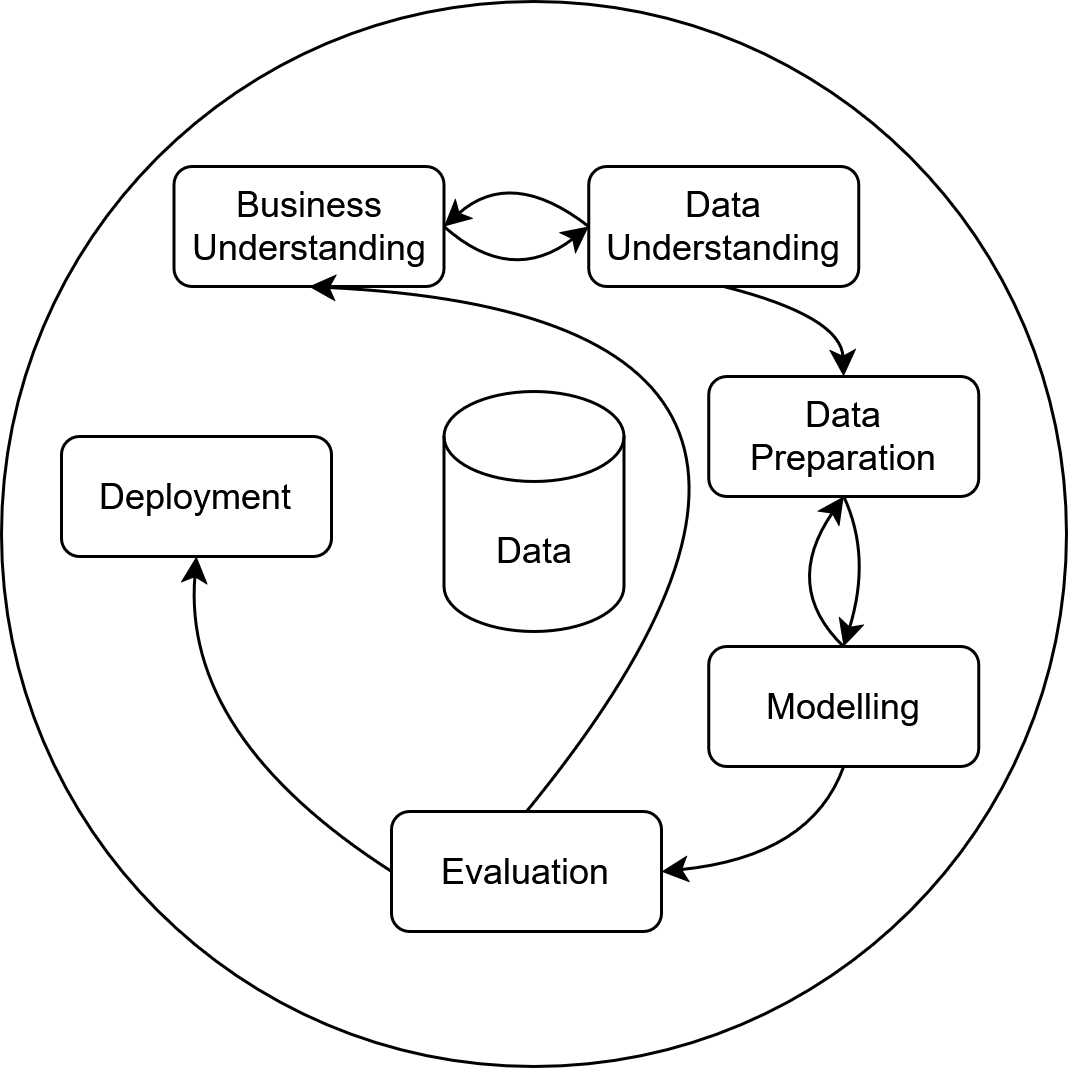
\includegraphics[width=.8\textwidth]{../images/crispdm.png}
	\caption{Proses dalam Metodologi \crisp{}}
	\label{fig:crisp-dm}
\end{figure}

\pagebreak

\crisp{} mencakup beberapa tahapan, yakni sebagai berikut:
